\documentclass[english,compress,aspectratio=43]{beamer}
\usefonttheme[onlymath]{serif} %Math font
\usepackage[english]{babel}

\usepackage[T1]{fontenc}
\usepackage[latin1]{inputenc}
\usepackage{lmodern}% http://ctan.org/pkg/lm To allow arbitrary font sizes
\usepackage{textpos}
\usepackage{mathtools} %Extension to amsmath
\usepackage{amsfonts,amssymb,dsfont}
\usepackage[font=footnotesize]{caption}
\usepackage{pifont}% http://ctan.org/pkg/pifont
\newcommand{\cmark}{\ding{51}}%
\newcommand{\xmark}{\ding{55}}%
\usepackage{graphicx}
\usepackage{epstopdf}
\usepackage{textcomp,gensymb} %degree symbol \degree
\usepackage{algorithm}
\usepackage{algpseudocode}
\usepackage{caption}
\captionsetup[figure]{labelformat=empty}

\usepackage[caption=false]{subfig}

\usepackage{algorithm}
\usepackage{algpseudocode}
\usepackage{algorithm}
\algrenewcommand\alglinenumber[1]{\tiny #1:}

\usepackage{tikz}
\usepackage[customcolors]{hf-tikz}

\tikzset{style green/.style={
    set fill color=green!50!lime!60,
    set border color=white,
  },
  style cyan/.style={
    set fill color=cyan!90!blue!60,
    set border color=white,
  },
  style orange/.style={
    set fill color=orange!80!red!60,
    set border color=white,
  },
  hor/.style={
    above left offset={-0.15,0.31},
    below right offset={0.15,-0.125},
    #1
  },
  ver/.style={
    above left offset={-0.1,0.3},
    below right offset={0.15,-0.15},
    #1
  }
}

\usepackage[customcolors,shadow,roundedcorners]{dynblocks}
\setbordercolor{blue!10}
\setshadowopacity{0.8}
\usepackage{environ}
\newsavebox\mybox

\NewEnviron{cdyn}[1]{%
    \sbox{\mybox}{$\BODY$}% \sbox{\mybox}{$\BODY$}
    \begin{center}
    \begin{dynblock}
    \opaqueblock<#1>[\wd\mybox]{\[\BODY\]}
    \end{dynblock}
    \end{center}
}{}%

\mode<presentation>
{
  \usetheme{Warsaw}
  %\usetheme{Malmoe}
  %\usetheme{Copenhagen}
  %\usetheme{Madrid}

  \setbeamercovered{transparent}
  \useoutertheme{infolines}
}

\usepackage{etoolbox}
\makeatletter
\patchcmd{\beamer@sectionintoc}{\vskip1.5em}{\vskip0.8em}{}{} %Hay que cambiar el segundo par�metro
\makeatother

\title[Breaking the (FAQin) badge]{Breaking the (FAQin) badge}
\author[Rodolfo Garc�a (kix)]{Rodolfo Garc�a Pe�as (kix)\\ {\tiny kix@kix.es | @thekix}} % (optional, use only with lots of authors)
\date[October 2019]{October 2019}

\AtBeginSection[]
{
  \begin{frame}<beamer>
   \frametitle{Outline}
    \tableofcontents[currentsection,hideothersubsections]
  \end{frame}
}

\begin{document}

\logo{\includegraphics[height=0.5cm]{images/faqin-just-for-fun.jpg}}

\begin{frame}
  \titlepage
  \begin{textblock*}{2cm}(0.5cm,-0.5cm)
\end{textblock*}
\begin{textblock*}{2cm}(8cm,-0.5cm)
\end{textblock*}
\end{frame}

\begin{frame}
  \frametitle{Outline}
  \tableofcontents[hideallsubsections]
\end{frame}

\section{Introduction}

\begin{frame}
  \frametitle{Introduction}
    \centering
    \includegraphics[width=0.62\textwidth]{images/faqin-badge-twitter.jpg}\\
    \begin{itemize}
      \item This badge was the present for the attendees to the last \textbf{FAQin Congress} (2019)
      \item The badge is an NFC card (tip: see the waves in the right area ;-) )
      \item We need read the card contents!! -> HW and SW tools
    \end{itemize}
\end{frame}

\section{NFC}

\begin{frame}
\frametitle{Reading the NFC Card}

\begin{columns}[t]
    \column{0.5\textwidth}
    \begin{center}
        \textbf{ACR122U}
        \vspace{0.2cm} \\
        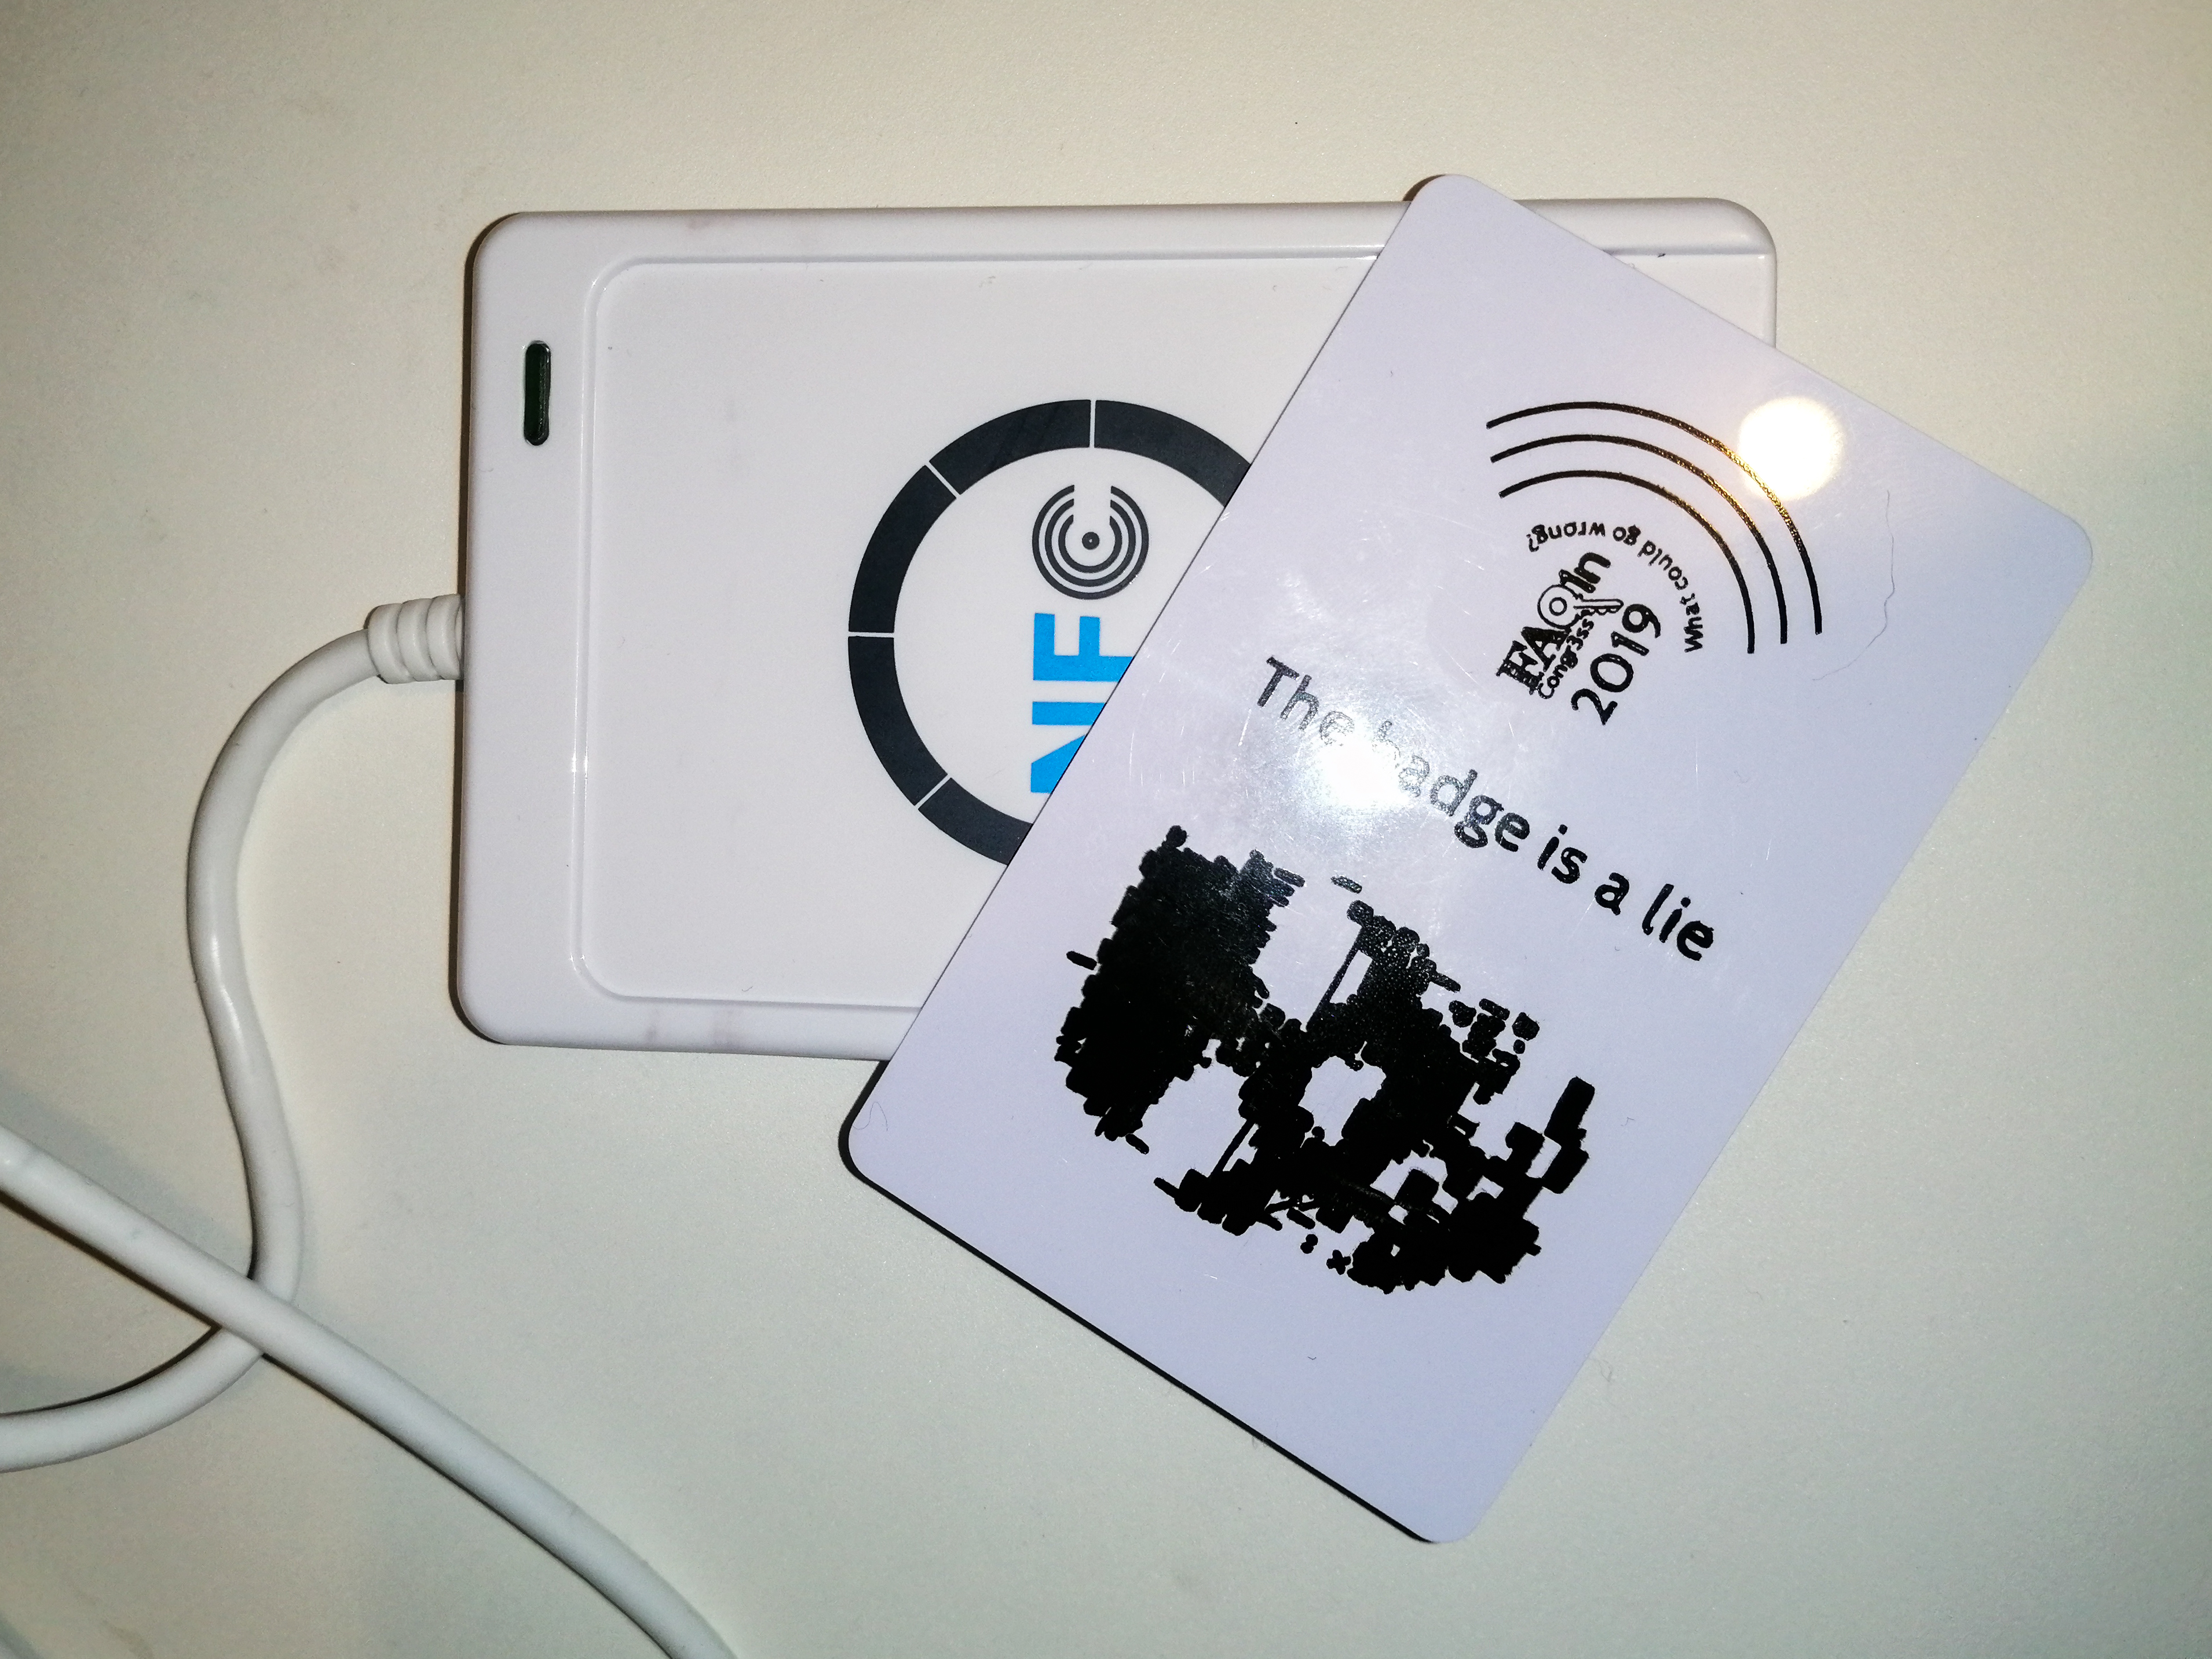
\includegraphics[width=0.9\textwidth]{images/IMG_20191020_222617.jpg}
    \end{center}

    \column{0.5\textwidth}
    \begin{center}
        \textbf{Proxmark}
        \vspace{0.2cm} \\
        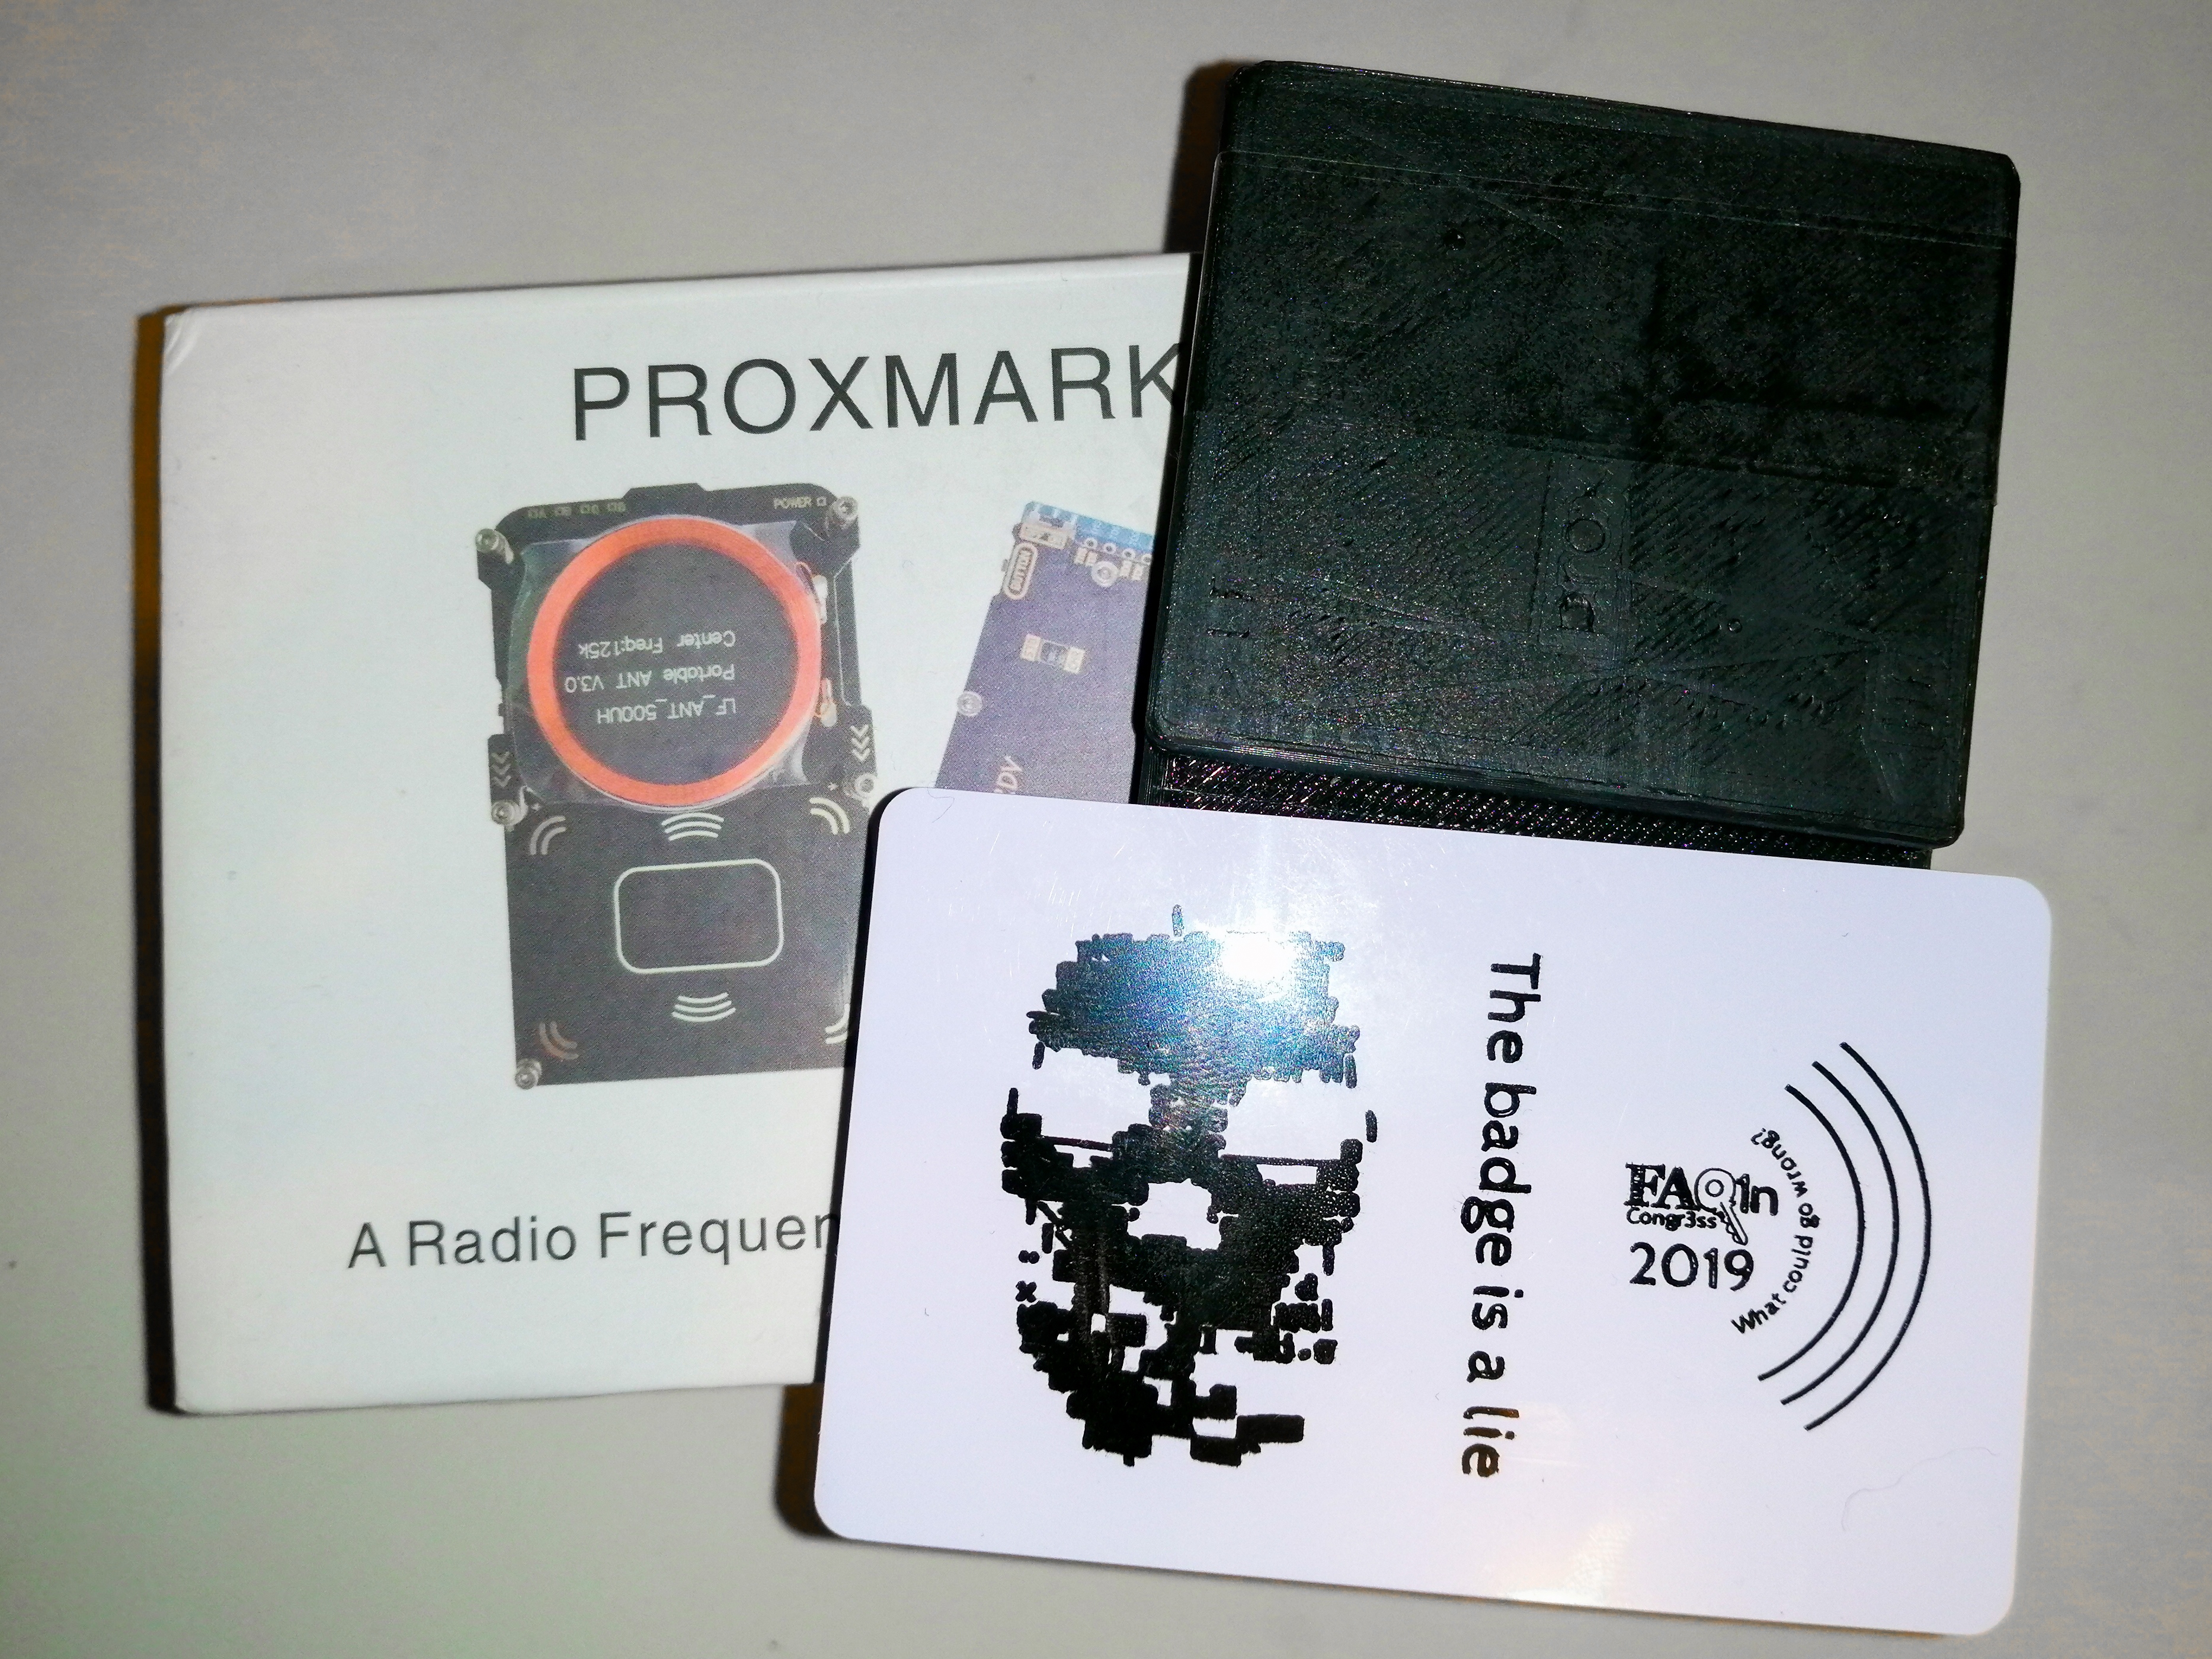
\includegraphics[width=0.9\textwidth]{images/IMG_20191020_222753.jpg}
    \end{center}
\end{columns}

\vspace{0.2cm}
\begin{block}{\textbf{Readers}}
\begin{itemize}
  \item You can use some NFC readers.
  \item I used ACR122U and Proxmark ('like') devices
\end{itemize}
\end{block}
\vspace{0.2cm}

\end{frame}

\begin{frame}[fragile]
\frametitle{Identify the NFC Card}

\vspace{0.2cm}
\begin{block}{\textbf{nfc-list}}
  \begin{itemize}
    \item Using nfc-list we can read the NFC Card info
    \item<2-> Card is an ISO 14443A, standard for RFID, 13.56 MHz
    \item<3-> This card is a MiFare Classic (MFC) Card
  \end{itemize}
\end{block}
\vspace{0.2cm}

  {\tiny
    \begin{verbatim}
kix@seahorse:~/src/nfc/faqin/script$ nfc-list -v
nfc-list uses libnfc 1.7.1
NFC device: ACS / ACR122U PICC Interface opened
1 ISO14443A passive target(s) found:
ISO/IEC 14443A (106 kbps) target:
    ATQA (SENS_RES): 00  04  
* UID size: single
* bit frame anticollision supported
       UID (NFCID1): 3a  92  ed  1a  
      SAK (SEL_RES): 08  
* Not compliant with ISO/IEC 14443-4
* Not compliant with ISO/IEC 18092

Fingerprinting based on MIFARE type Identification Procedure:
* MIFARE Classic 1K
* MIFARE Plus (4 Byte UID or 4 Byte RID) 2K, Security level 1
* SmartMX with MIFARE 1K emulation
    \end{verbatim}
  }

\end{frame}

\begin{frame}
  \frametitle{MiFare Classic structure 1/2}
    \begin{block}{\textbf{MFC 1K structure}}
      \begin{itemize}
        \item 16 sectors of 4 blocks of 16 bytes:
        \item Every sector (4 blocks) include:
        \begin{itemize}
          \item 3 data blocks: 48 bytes
          \item 1 card info block: 2 passwords (6B + 6B) + access bytes (4B)
        \end{itemize}
        \item First block in sector zero is the manufacturer block ("not writable"). It includes:
        \begin{itemize}
          \item Card ID (UUID), 4 bytes
          \item ATQA: Answer To reQuest Action (00 04 to MFC), 2 bytes
          \item SAK: Select AcKnowledge (08 to MFC), 1 byte
          \item CHECK: Checksum, 1 byte
          \item 2 * 6 bytes of passwords + access data
        \end{itemize}
        \item Data:
        \begin{itemize}
          \item Max user data: 752 bytes: (1sec * 2blk + 15sec * 3blk) * 16 bytes
          \item Usually, empty blocks contains zeroes
        \end{itemize}
      \end{itemize}
    \end{block}
  {\let\thefootnote\relax\footnote{https://www.nxp.com/docs/en/application-note/AN10833.pdf}}
\end{frame}

\begin{frame}
  \frametitle{MiFare Classic structure 2/2}
  \begin{block}{\textbf{Example:}}
    \begin{itemize}
      \item This is an example with the FAQin badge (yes, we need read it first)
    \end{itemize}
  \end{block}
  \begin{center}
      \includegraphics[width=0.7\textwidth]{images/shot_mifare_header.png}
  \end{center}
\end{frame}

\begin{frame}
  \frametitle{Read the NFC Card}
  \begin{block}{}
    Reading the badge...
  \end{block}
\end{frame}

\begin{frame}[fragile]
  \frametitle{Read the card using \textbf{mfoc} 1/4}
  \begin{block}{\textbf{mfoc}}
    \begin{itemize}
      \item \texttt{\textbf{mfoc}} is an utility to read MFC cards
      \item<2-> It uses default passwords or dictionaries to read the contents
    \end{itemize}
  \end{block}

  {\scriptsize
    \begin{verbatim}
kix@seahorse:~/src/nfc/faqin/script$ mfoc -h
Usage: mfoc [-h] [-k key] [-f file] ... [-P probnum] [-T tolerance] [-O output]

  h     print this help and exit
  k     try the specified key in addition to the default keys
  f     parses a file of keys to add in addition to the default keys 
  P     number of probes per sector, instead of default of 20
  T     nonce tolerance half-range, instead of default of 20
        (i.e., 40 for the total range, in both directions)
  O     file in which the card contents will be written (REQUIRED)
  D     file in which partial card info will be written in case PRNG is not... 

Example: mfoc -O mycard.mfd
Example: mfoc -k ffffeeeedddd -O mycard.mfd
Example: mfoc -f keys.txt -O mycard.mfd
Example: mfoc -P 50 -T 30 -O mycard.mfd

    \end{verbatim}
  }

\end{frame}

\begin{frame}[fragile]
  \frametitle{Read the card using \textbf{mfoc} 2/4}
  \begin{block}{\textbf{mfoc}}
    \begin{itemize}
      \item Trying \texttt{\textbf{mfoc}} with default passwords:
    \end{itemize}
  \end{block}

  {\tiny
    \begin{verbatim}
kix@seahorse:~/src/nfc/faqin/script$ mfoc -P 50 -T 30 -O mycard.mfd
-----8<----- snip -----8<-----

Try to authenticate to all sectors with default keys...
Symbols: '.' no key found, '/' A key found, '\' B key found, 'x' both keys found
[Key: ffffffffffff] -> [................]
[Key: a0a1a2a3a4a5] -> [................]
[Key: d3f7d3f7d3f7] -> [................]
[Key: 000000000000] -> [................]
[Key: b0b1b2b3b4b5] -> [................]
[Key: 4d3a99c351dd] -> [................]
[Key: 1a982c7e459a] -> [................]
[Key: aabbccddeeff] -> [................]
[Key: 714c5c886e97] -> [................]
[Key: 587ee5f9350f] -> [................]
[Key: a0478cc39091] -> [................]
[Key: 533cb6c723f6] -> [................]
[Key: 8fd0a4f256e9] -> [................]

-----8<----- snip -----8<-----
    \end{verbatim}
  }

\end{frame}

\begin{frame}[fragile]
  \frametitle{Read the card using \textbf{mfoc} 3/4}
  \begin{block}{\textbf{mfoc}}
    \begin{itemize}
      \item Or using with default dictionaries, like [1]
    \end{itemize}
  \end{block}

  {\tiny
    \begin{verbatim}
kix@seahorse:~/src/nfc/faqin/script$ mfoc -P 50 -T 30 -O mycard.mfd
-----8<----- snip -----8<-----

Sector 00 - Unknown Key A               Unknown Key B
Sector 01 - Unknown Key A               Unknown Key B
Sector 02 - Unknown Key A               Unknown Key B
Sector 03 - Unknown Key A               Unknown Key B
Sector 04 - Unknown Key A               Unknown Key B
Sector 05 - Unknown Key A               Unknown Key B
Sector 06 - Unknown Key A               Unknown Key B
Sector 07 - Unknown Key A               Unknown Key B
Sector 08 - Unknown Key A               Unknown Key B
Sector 09 - Unknown Key A               Unknown Key B
Sector 10 - Unknown Key A               Unknown Key B
Sector 11 - Unknown Key A               Unknown Key B
Sector 12 - Unknown Key A               Unknown Key B
Sector 13 - Unknown Key A               Unknown Key B
Sector 14 - Unknown Key A               Unknown Key B
Sector 15 - Unknown Key A               Unknown Key B
mfoc: ERROR: 

No sector encrypted with the default key has been found, exiting..
    \end{verbatim}
  }

  \tiny{[1] https://github.com/ikarus23/MifareClassicTool/blob/master/Mifare\%20Classic\%20Tool/app/src/main/assets/key-files/extended-std.keys}
\end{frame}

\begin{frame}[fragile]
  \frametitle{Read the card using \textbf{mfoc} 4/4}
  \begin{block}{\textbf{mfoc}}
    \begin{itemize}
      \item It returns an unsuccessful result, unable to read the card
      \item We need other methods
    \end{itemize}
  \end{block}

\end{frame}

\begin{frame}[fragile]
  \frametitle{Read the card using \textbf{mfcuk}}
  \begin{block}{\textbf{mfcuk}}
    \begin{itemize}
      \item \texttt{\textbf{mfcuk}} MiFare Classic Universal toolKit
      \item<2-> \texttt{\textbf{mfcuk}} is another utility to read MFC cards
      \item<3-> It uses different methods to read the card info:
      \begin{itemize}
        \item<3-> Default passwords or dictionaries
        \item<3-> Proxmark sniffed conversations
        \item<3-> Nested, hardnested and darkside attacks
      \end{itemize}
    \end{itemize}
  \end{block}
\end{frame}

\begin{frame}[fragile]
  \frametitle{Read the card using \textbf{mfcuk}}
  \begin{block}{\textbf{mfcuk}}
    \begin{itemize}
      \item Attacks using default passwords and dictionaries is like with \textbf{mfoc}: :-(
      \item nested and hardnested attacks needs at least one key: :'(
      \item Then... darkside attack!
    \end{itemize}
  \end{block}
\end{frame}

\begin{frame}[fragile]
  \frametitle{Read the card using \textbf{mfcuk}}
  \begin{block}{\textbf{Darkside Attack}}
    \begin{itemize}
      \item Is a "brute force" attack
      \item You can run it with something like these:
    \end{itemize}
  \end{block}

  {\tiny
    \begin{verbatim}
$ mfcuk -C -R 0:A -s 50 -S 50 -O faqin.dmp -v 3
mfcuk - 0.3.8
Mifare Classic DarkSide Key Recovery Tool - 0.3
...
-----------------------------------------------------
Let me entertain you!
    uid: 3a92ed1a
   type: 08
    key: 000000000000
  block: 03
diff Nt: 0
  auths: 0
-----------------------------------------------------
...
    \end{verbatim}
  }

  \begin{block}{}
    It takes some time... about 20-30 minutes
  \end{block}

\end{frame}

\begin{frame}[fragile]
  \frametitle{Read the card using \textbf{mfcuk}}

  \begin{block}{}
    It takes some time more... about 1-3 hours
  \end{block}

  {\tiny
    \begin{verbatim}
...
-----------------------------------------------------
Let me entertain you!
    uid: 3a92ed1a
   type: 08
    key: 000000000000
  block: 03
diff Nt: 1416
  auths: 20851
-----------------------------------------------------

-----------------------------------------------------
Let me entertain you!
    uid: 3a92ed1a
   type: 08
    key: 000000000000
  block: 03
diff Nt: 1480
  auths: 32851
-----------------------------------------------------
...
    \end{verbatim}
  }
\end{frame}

\begin{frame}[fragile]
  \frametitle{Read the card using \textbf{mfcuk}}

  \begin{block}{}
    Three/four days later... wtf! \\ It doesn't finish! (20 min expected)
  \end{block}
\end{frame}

\begin{frame}[fragile]
  \frametitle{Read the card using \textbf{Proxmark}}

  \begin{block}{}
    \textbf{Proxmark} time...
  \end{block}
\end{frame}

\begin{frame}[fragile]
  \frametitle{Read the card using \textbf{Proxmark}}

  \begin{block}{DarkSide with Proxmark}
    Trying the Darkside attack using Proxmark:
  \end{block}

  {\tiny
    \begin{verbatim}
proxmark3> hf mf mifare
-------------------------------------------------------------------------
Executing command. Expected execution time: 25sec on average
Press button on the proxmark3 device to abort both proxmark3 and client.
-------------------------------------------------------------------------
.....Card is not vulnerable to Darkside attack (its random number generator seems to be based on the wellknown
generating polynomial with 16 effective bits only, but shows unexpected behaviour.
proxmark3>
...
    \end{verbatim}
  }
\end{frame}

\begin{frame}[fragile]
  \frametitle{Bruce force the NFC card?}
  \begin{block}{}
    \begin{itemize}
      \item There is no real option with standard tools
      \item I created a modified version of \textbf{mfoc} to make brute force, but it takes too much time.
    \end{itemize}
  \end{block}

  \begin{block}{}
    \begin{itemize}
      \item Is not possible to break it. Perhaps the new Proxmark?
      \item Game ends here... waiting my bruteforce attack...
    \end{itemize}
  \end{block}
\end{frame}

\begin{frame}
  \frametitle{WhiskyLeaks or TwitterLeaks}
  \begin{block}{}
      40 days later...
  \end{block}
    \centering
    \includegraphics[width=0.62\textwidth]{images/twitter-key.png}\\
\end{frame}

\begin{frame}
  \frametitle{Dump card keys}
  \begin{block}{}
      We have one key. We can recover all keys with this key using \textbf{mfoc}
  \end{block}
\end{frame}

\begin{frame}[fragile]
  \frametitle{Dump card keys}
  \begin{block}{Dump the keys using \textbf{mfoc}}
    \begin{itemize}
      \item With one key (666dd3de6cc1) is possible to recover all keys and dump the badge data
      \item We run: \texttt{mfoc -k 666dd3de6cc1 -O 20190907\_faqin.mfc}
    \end{itemize}
  \end{block}

  {\tiny
    \begin{verbatim}
Sector 00 - Key A: 564a0c9b9ef7 - Key B: 043af4e1e893
Sector 01 - Key A: 2c83b0993c87 - Key B: 497ce4368088
Sector 02 - Key A: 77d7f74b4bc3 - Key B: 447503e3eba7
Sector 03 - Key A: c9d995ec939a - Key B: 6b2c8b1a1d67
Sector 04 - Key A: 02662056aecd - Key B: 666dd3de6cc1
Sector 05 - Key A: 37ab2cb03ec3 - Key B: fbdcb5468b84
Sector 06 - Key A: 8749f086d780 - Key B: a941914a824e
Sector 07 - Key A: 619585c75e3c - Key B: 349486e5b52f
Sector 08 - Key A: 704205d57dd4 - Key B: 2c59d41ecb80
Sector 09 - Key A: 020aa9d31304 - Key B: cc3e710e8bd6
Sector 10 - Key A: bd2baa246881 - Key B: 6cdb55b3603b
Sector 11 - Key A: dd27e3b0af89 - Key B: e3fab0a0f1b5
Sector 12 - Key A: 9a3cbca3cc9f - Key B: f8aa5d7591bc
Sector 13 - Key A: 5c1045cce0be - Key B: fe79d0fbb4ec
Sector 14 - Key A: 868009686575 - Key B: 46f651f19c85
Sector 15 - Key A: d86ca4cd9921 - Key B: 652df83017c6
    \end{verbatim}
  }
\end{frame}

\begin{frame}[fragile]
  \frametitle{Dump card contents}
  \begin{block}{}
    Now we have the data in \texttt{20190907\_faqin.mfc}
  \end{block}

\begin{columns}
\column{0.45\textwidth}
  {\fontsize{4}{4}\selectfont
    \begin{verbatim}
kix@seahorse:~/src/nfc/faqin/script$ hexdump -vC 20190907_faqin.mfc
0000  3a 92 ed 1a 5f 08 04 00  62 63 64 65 66 67 68 69  |:..._...bcdefghi|
0010  ab bc 1c 0e 86 e6 0e 97  e6 0e c5 e7 59 08 9b d6  |............Y...|
0020  26 5f e6 e7 15 4c 59 38  9b 5f c6 e6 15 4c 66 1f  |&_...LY8._...Lf.|
0030  56 4a 0c 9b 9e f7 08 77  8f 69 04 3a f4 e1 e8 93  |VJ.....w.i.:....|
0040  fe 92 05 58 89 9b 0e 8e  e6 5e 08 9b 0e 93 e6 0e  |...X.....^......|
0050  8d e6 58 08 9b 66 da e6  92 34 58 08 9b 59 94 9b  |..X..f...4X..Y..|
0060  0e 71 e6 e9 64 1a e6 59  90 9b 0e 6b e6 59 98 9b  |.q..d..Y...k.Y..|
0070  2c 83 b0 99 3c 87 08 77  8f 69 49 7c e4 36 80 88  |,...<..w.iI|.6..|
0080  e9 64 02 e6 59 9c 9b 0e  66 e6 59 77 9b e9 64 31  |.d..Y...f.Yw..d1|
0090  e6 0e 6b e6 0d 40 5e e5  e6 2b f6 0e e7 e6 25 5e  |..k..@^..+....%^|
00a0  c6 ef 5f e6 f6 55 e4 2b  f6 25 0e 0f 19 5e c6 ef  |.._..U.+.%...^..|
00b0  77 d7 f7 4b 4b c3 08 77  8f 69 44 75 03 e3 eb a7  |w..KK..w.iDu....|
00c0  5f b6 e6 55 66 2b f6 58  84 9b 0e e2 e6 0e eb e6  |_..Uf+.X........|
00d0  25 52 e8 4a da e6 92 e2  2b f6 0d 11 25 58 b9 9b  |%R.J....+...%X..|
00e0  0e 08 19 25 86 6f 21 d7  2f 0e f8 e6 da eb 92 f3  |...%.o!./.......|
00f0  c9 d9 95 ec 93 9a 08 77  8f 69 6b 2c 8b 1a 1d 67  |.......w.ik,...g|
0100  da c6 94 13 0d e6 86 52  e8 2b f6 87 4c a7 65 1f  |.......R.+..L.e.|
0110  f6 e9 6a 02 19 d7 26 4c  87 25 86 5e e6 f6 2b f0  |..j...&L.%.^..+.|
0120  45 3e 9a 87 47 3e 9a 25  e6 e6 86 6c e2 6c fb de  |E>..G>.%...l.l..|
0130  02 66 20 56 ae cd 08 77  8f 69 66 6d d3 de 6c c1  |.f V...w.ifm..l.|
0140  3e 93 ee da e6 92 e1 a0  a1 0d 16 87 1e 25 87 1f  |>............%..|
0150  25 6c f2 6c 92 e7 d7 10  5f ee e6 58 28 9b df 28  |%l.l...._..X(..(|
0160  92 f6 6d e2 d6 12 d6 36  0e eb e6 0e 5a 19 a0 a0  |..m....6....Z...|
0170  37 ab 2c b0 3e c3 08 77  8f 69 fb dc b5 46 8b 84  |7.,.>..w.i...F..|
0180  04 0a 0e fc e6 0e 12 18  86 6f 27 56 50 00 a5 6f  |.........o'VP..o|
0190  2e 00 a4 6e 06 00 a4 02  87 ea e5 00 87 87 25 86  |...n..........%.|
01a0  02 87 c2 1a 00 87 87 25  6f 18 0e b2 19 0e bb 19  |.......%o.......|
01b0  87 49 f0 86 d7 80 08 77  8f 69 a9 41 91 4a 82 4e  |.I.....w.i.A.J.N|
01c0  0e 2f 18 5e e7 b5 d7 3d  2b f3 5e e8 b5 d7 3d 5f  |./.^...=+.^...=_|
01d0  e4 e7 2b f3 5e e1 b5 5d  e7 e6 5f e5 e6 2b f3 ec  |..+.^..].._..+..|
01e0  eb e6 a0 a7 b7 8f 88 c6  a9 b5 c6 90 d2 d4 e6 d8  |................|
01f0  61 95 85 c7 5e 3c 08 77  8f 69 34 94 86 e5 b5 2f  |a...^<.w.i4..../|
    \end{verbatim}
  }

\column{0.45\textwidth}
  {\fontsize{4}{4}\selectfont
    \begin{verbatim}

0200  c6 e6 8e 8a 92 e6 8e 8a  96 e6 8f 88 80 e6 85 8b  |................|
0210  82 dc c6 8e 8a 92 ca c6  8e 8a 96 ca c6 8f 88 80  |................|
0220  e6 ab 9d a9 b5 9b a5 c6  cb c6 ab af a0 a7 b4 a3  |................|
0230  70 42 05 d5 7d d4 08 77  8f 69 2c 59 d4 1e cb 80  |pB..}..w.i,Y....|
0240  c6 a9 b5 c6 a5 8e 87 8a  8a 83 88 81 83 e6 a4 9f  |................|
0250  c6 a6 84 8f 92 95 88 8f  96 83 94 e6 ae 83 8a 8a  |................|
0260  89 c6 91 89 94 8a 82 c6  aa 87 94 87 c7 e6 5b c6  |..............[.|
0270  02 0a a9 d3 13 04 08 77  8f 69 cc 3e 71 0e 8b d6  |.......w.i.>q...|
0280  1c dd 5b c6 a3 c5 94 c1  ef c2 2f c7 5b c6 e6 e6  |..[......./.[...|
0290  e6 e6 e6 e6 e6 e6 e6 e6  e6 e6 e6 e6 e6 e6 e6 e6  |................|
02a0  e6 e6 e6 e6 e6 e6 e6 e6  e6 e6 e6 e6 e6 e6 b3 4c  |...............L|
02b0  bd 2b aa 24 68 81 08 77  8f 69 6c db 55 b3 60 3b  |.+.$h..w.il.U.`;|
02c0  e6 e6 e6 e6 e6 e6 e6 e6  e6 e6 e6 e6 e6 e6 e6 e6  |................|
02d0  8d 83 9f db d6 9e d0 df  e6 e6 e6 e6 e6 e6 e6 e6  |................|
02e0  fe ea e2 fa a2 fc f6 fc  fb ea e2 a2 e6 bc b7 b9  |................|
02f0  dd 27 e3 b0 af 89 08 77  8f 69 e3 fa b0 a0 f1 b5  |.'.....w.i......|
0300  af a2 fc e0 fa e1 eb e7  f8 af ff ec fc ff e4 af  |................|
0310  a2 e9 eb ee af ed e0 e0  fb a1 ed e6 e1 e6 e6 e6  |................|
0320  00 00 00 00 00 00 00 00  00 00 00 00 00 00 00 00  |................|
0330  9a 3c bc a3 cc 9f 08 77  8f 69 f8 aa 5d 75 91 bc  |.<.....w.i..]u..|
0340  00 00 00 00 00 00 00 00  00 00 00 00 00 00 00 00  |................|
0350  00 00 00 00 00 00 00 00  00 00 00 00 00 00 00 00  |................|
0360  00 00 00 00 00 00 00 00  00 00 00 00 00 00 00 00  |................|
0370  5c 10 45 cc e0 be 08 77  8f 69 fe 79 d0 fb b4 ec  |\.E....w.i.y....|
0380  00 00 00 00 00 00 00 00  00 00 00 00 00 00 00 00  |................|
0390  00 00 00 00 00 00 00 00  00 00 00 00 00 00 00 00  |................|
03a0  00 00 00 00 00 00 00 00  00 00 00 00 00 00 00 00  |................|
03b0  86 80 09 68 65 75 08 77  8f 69 46 f6 51 f1 9c 85  |...heu.w.iF.Q...|
03c0  00 00 00 00 00 00 00 00  00 00 00 00 00 00 00 00  |................|
03d0  00 00 00 00 00 00 00 00  00 00 00 00 00 00 00 00  |................|
03e0  00 00 00 00 00 00 00 00  00 00 00 00 00 00 00 00  |................|
03f0  d8 6c a4 cd 99 21 08 77  8f 69 65 2d f8 30 17 c6  |.l...!.w.ie-.0..|
    \end{verbatim}
  }
\end{columns}
\end{frame}

\section{Data analysis}

\begin{frame}
  \frametitle{Card dump}
  \begin{block}{}
    This is the dump (hex), including the keys (red), access control (green),...
  \end{block}

    \centering
    \includegraphics[width=0.48\textwidth]{images/card_dump_full.png}\\
\end{frame}

\begin{frame}[fragile]
  \frametitle{Card dump - Only data}
  \begin{block}{}
    This is the dump (hex). Only data.
  \end{block}

\begin{columns}
\column{0.45\textwidth}
  {\fontsize{4}{4}\selectfont
    \begin{verbatim}
0010  ab bc 1c 0e 86 e6 0e 97  e6 0e c5 e7 59 08 9b d6  |............Y...|
0020  26 5f e6 e7 15 4c 59 38  9b 5f c6 e6 15 4c 66 1f  |&_...LY8._...Lf.|
0040  fe 92 05 58 89 9b 0e 8e  e6 5e 08 9b 0e 93 e6 0e  |...X.....^......|
0050  8d e6 58 08 9b 66 da e6  92 34 58 08 9b 59 94 9b  |..X..f...4X..Y..|
0060  0e 71 e6 e9 64 1a e6 59  90 9b 0e 6b e6 59 98 9b  |.q..d..Y...k.Y..|
0080  e9 64 02 e6 59 9c 9b 0e  66 e6 59 77 9b e9 64 31  |.d..Y...f.Yw..d1|
0090  e6 0e 6b e6 0d 40 5e e5  e6 2b f6 0e e7 e6 25 5e  |..k..@^..+....%^|
00a0  c6 ef 5f e6 f6 55 e4 2b  f6 25 0e 0f 19 5e c6 ef  |.._..U.+.%...^..|
00c0  5f b6 e6 55 66 2b f6 58  84 9b 0e e2 e6 0e eb e6  |_..Uf+.X........|
00d0  25 52 e8 4a da e6 92 e2  2b f6 0d 11 25 58 b9 9b  |%R.J....+...%X..|
00e0  0e 08 19 25 86 6f 21 d7  2f 0e f8 e6 da eb 92 f3  |...%.o!./.......|
0100  da c6 94 13 0d e6 86 52  e8 2b f6 87 4c a7 65 1f  |.......R.+..L.e.|
0110  f6 e9 6a 02 19 d7 26 4c  87 25 86 5e e6 f6 2b f0  |..j...&L.%.^..+.|
0120  45 3e 9a 87 47 3e 9a 25  e6 e6 86 6c e2 6c fb de  |E>..G>.%...l.l..|
0140  3e 93 ee da e6 92 e1 a0  a1 0d 16 87 1e 25 87 1f  |>............%..|
0150  25 6c f2 6c 92 e7 d7 10  5f ee e6 58 28 9b df 28  |%l.l...._..X(..(|
0160  92 f6 6d e2 d6 12 d6 36  0e eb e6 0e 5a 19 a0 a0  |..m....6....Z...|
0180  04 0a 0e fc e6 0e 12 18  86 6f 27 56 50 00 a5 6f  |.........o'VP..o|
0190  2e 00 a4 6e 06 00 a4 02  87 ea e5 00 87 87 25 86  |...n..........%.|
01a0  02 87 c2 1a 00 87 87 25  6f 18 0e b2 19 0e bb 19  |.......%o.......|
01c0  0e 2f 18 5e e7 b5 d7 3d  2b f3 5e e8 b5 d7 3d 5f  |./.^...=+.^...=_|
01d0  e4 e7 2b f3 5e e1 b5 5d  e7 e6 5f e5 e6 2b f3 ec  |..+.^..].._..+..|
01e0  eb e6 a0 a7 b7 8f 88 c6  a9 b5 c6 90 d2 d4 e6 d8  |................|
0200  c6 e6 8e 8a 92 e6 8e 8a  96 e6 8f 88 80 e6 85 8b  |................|
0210  82 dc c6 8e 8a 92 ca c6  8e 8a 96 ca c6 8f 88 80  |................|
0220  e6 ab 9d a9 b5 9b a5 c6  cb c6 ab af a0 a7 b4 a3  |................|
0240  c6 a9 b5 c6 a5 8e 87 8a  8a 83 88 81 83 e6 a4 9f  |................|
0250  c6 a6 84 8f 92 95 88 8f  96 83 94 e6 ae 83 8a 8a  |................|
0260  89 c6 91 89 94 8a 82 c6  aa 87 94 87 c7 e6 5b c6  |..............[.|
0280  1c dd 5b c6 a3 c5 94 c1  ef c2 2f c7 5b c6 e6 e6  |..[......./.[...|
0290  e6 e6 e6 e6 e6 e6 e6 e6  e6 e6 e6 e6 e6 e6 e6 e6  |................|
02a0  e6 e6 e6 e6 e6 e6 e6 e6  e6 e6 e6 e6 e6 e6 b3 4c  |...............L|
02c0  e6 e6 e6 e6 e6 e6 e6 e6  e6 e6 e6 e6 e6 e6 e6 e6  |................|
02d0  8d 83 9f db d6 9e d0 df  e6 e6 e6 e6 e6 e6 e6 e6  |................|
02e0  fe ea e2 fa a2 fc f6 fc  fb ea e2 a2 e6 bc b7 b9  |................|
0300  af a2 fc e0 fa e1 eb e7  f8 af ff ec fc ff e4 af  |................|
0310  a2 e9 eb ee af ed e0 e0  fb a1 ed e6 e1 e6 e6 e6  |................|
0320  00 00 00 00 00 00 00 00  00 00 00 00 00 00 00 00  |................| ----> Empty!
0340  00 00 00 00 00 00 00 00  00 00 00 00 00 00 00 00  |................| ----> Empty!
0350  00 00 00 00 00 00 00 00  00 00 00 00 00 00 00 00  |................| ----> Empty!
0360  00 00 00 00 00 00 00 00  00 00 00 00 00 00 00 00  |................| ----> Empty!
0380  00 00 00 00 00 00 00 00  00 00 00 00 00 00 00 00  |................| ----> Empty!
0390  00 00 00 00 00 00 00 00  00 00 00 00 00 00 00 00  |................| ----> Empty!
03a0  00 00 00 00 00 00 00 00  00 00 00 00 00 00 00 00  |................| ----> Empty!
03c0  00 00 00 00 00 00 00 00  00 00 00 00 00 00 00 00  |................| ----> Empty!
03d0  00 00 00 00 00 00 00 00  00 00 00 00 00 00 00 00  |................| ----> Empty!
03e0  00 00 00 00 00 00 00 00  00 00 00 00 00 00 00 00  |................| ----> Empty!
    \end{verbatim}
  }
\end{columns}
\end{frame}

\begin{frame}[fragile]
  \frametitle{Card dump - Valid data only}
  \begin{block}{}
    Valid data only, without the 00's (probably no info)
  \end{block}


\begin{columns}
\column{0.45\textwidth}
  {\fontsize{4}{4}\selectfont
    \begin{verbatim}
0010  ab bc 1c 0e 86 e6 0e 97  e6 0e c5 e7 59 08 9b d6  |............Y...|
0020  26 5f e6 e7 15 4c 59 38  9b 5f c6 e6 15 4c 66 1f  |&_...LY8._...Lf.|
0040  fe 92 05 58 89 9b 0e 8e  e6 5e 08 9b 0e 93 e6 0e  |...X.....^......|
0050  8d e6 58 08 9b 66 da e6  92 34 58 08 9b 59 94 9b  |..X..f...4X..Y..|
0060  0e 71 e6 e9 64 1a e6 59  90 9b 0e 6b e6 59 98 9b  |.q..d..Y...k.Y..|
0080  e9 64 02 e6 59 9c 9b 0e  66 e6 59 77 9b e9 64 31  |.d..Y...f.Yw..d1|
0090  e6 0e 6b e6 0d 40 5e e5  e6 2b f6 0e e7 e6 25 5e  |..k..@^..+....%^|
00a0  c6 ef 5f e6 f6 55 e4 2b  f6 25 0e 0f 19 5e c6 ef  |.._..U.+.%...^..|
00c0  5f b6 e6 55 66 2b f6 58  84 9b 0e e2 e6 0e eb e6  |_..Uf+.X........|
00d0  25 52 e8 4a da e6 92 e2  2b f6 0d 11 25 58 b9 9b  |%R.J....+...%X..|
00e0  0e 08 19 25 86 6f 21 d7  2f 0e f8 e6 da eb 92 f3  |...%.o!./.......|
0100  da c6 94 13 0d e6 86 52  e8 2b f6 87 4c a7 65 1f  |.......R.+..L.e.|
0110  f6 e9 6a 02 19 d7 26 4c  87 25 86 5e e6 f6 2b f0  |..j...&L.%.^..+.|
0120  45 3e 9a 87 47 3e 9a 25  e6 e6 86 6c e2 6c fb de  |E>..G>.%...l.l..|
0140  3e 93 ee da e6 92 e1 a0  a1 0d 16 87 1e 25 87 1f  |>............%..|
0150  25 6c f2 6c 92 e7 d7 10  5f ee e6 58 28 9b df 28  |%l.l...._..X(..(|
0160  92 f6 6d e2 d6 12 d6 36  0e eb e6 0e 5a 19 a0 a0  |..m....6....Z...|
0180  04 0a 0e fc e6 0e 12 18  86 6f 27 56 50 00 a5 6f  |.........o'VP..o|
0190  2e 00 a4 6e 06 00 a4 02  87 ea e5 00 87 87 25 86  |...n..........%.|
01a0  02 87 c2 1a 00 87 87 25  6f 18 0e b2 19 0e bb 19  |.......%o.......|
01c0  0e 2f 18 5e e7 b5 d7 3d  2b f3 5e e8 b5 d7 3d 5f  |./.^...=+.^...=_|
01d0  e4 e7 2b f3 5e e1 b5 5d  e7 e6 5f e5 e6 2b f3 ec  |..+.^..].._..+..|
01e0  eb e6 a0 a7 b7 8f 88 c6  a9 b5 c6 90 d2 d4 e6 d8  |................|
0200  c6 e6 8e 8a 92 e6 8e 8a  96 e6 8f 88 80 e6 85 8b  |................|
0210  82 dc c6 8e 8a 92 ca c6  8e 8a 96 ca c6 8f 88 80  |................|
0220  e6 ab 9d a9 b5 9b a5 c6  cb c6 ab af a0 a7 b4 a3  |................|
0240  c6 a9 b5 c6 a5 8e 87 8a  8a 83 88 81 83 e6 a4 9f  |................|
0250  c6 a6 84 8f 92 95 88 8f  96 83 94 e6 ae 83 8a 8a  |................|
0260  89 c6 91 89 94 8a 82 c6  aa 87 94 87 c7 e6 5b c6  |..............[.|
0280  1c dd 5b c6 a3 c5 94 c1  ef c2 2f c7 5b c6 e6 e6  |..[......./.[...|
0290  e6 e6 e6 e6 e6 e6 e6 e6  e6 e6 e6 e6 e6 e6 e6 e6  |................| <---- e6 e6 :-?
02a0  e6 e6 e6 e6 e6 e6 e6 e6  e6 e6 e6 e6 e6 e6 b3 4c  |...............L|
02c0  e6 e6 e6 e6 e6 e6 e6 e6  e6 e6 e6 e6 e6 e6 e6 e6  |................| <---- e6 e6 :-?
02d0  8d 83 9f db d6 9e d0 df  e6 e6 e6 e6 e6 e6 e6 e6  |................|
02e0  fe ea e2 fa a2 fc f6 fc  fb ea e2 a2 e6 bc b7 b9  |................|
0300  af a2 fc e0 fa e1 eb e7  f8 af ff ec fc ff e4 af  |................|
0310  a2 e9 eb ee af ed e0 e0  fb a1 ed e6 e1 e6 e6 e6  |................|
    \end{verbatim}
  }
\end{columns}
\end{frame}

\begin{frame}[fragile]
  \frametitle{Discovering data}

  \begin{block}{Looking the ciphered info}
    \begin{itemize}
      \item We can see a lot of "e6" in the end of the valid data
      \item Probably these info is "00", so we can apply an XOR
    \end{itemize}
  \end{block}

\begin{columns}
\column{0.45\textwidth}
  {\fontsize{4}{4}\selectfont
    \begin{verbatim}
01d0  e4 e7 2b f3 5e e1 b5 5d  e7 e6 5f e5 e6 2b f3 ec  |..+.^..].._..+..|
01e0  eb e6 a0 a7 b7 8f 88 c6  a9 b5 c6 90 d2 d4 e6 d8  |................|
0200  c6 e6 8e 8a 92 e6 8e 8a  96 e6 8f 88 80 e6 85 8b  |................|
0210  82 dc c6 8e 8a 92 ca c6  8e 8a 96 ca c6 8f 88 80  |................|
0220  e6 ab 9d a9 b5 9b a5 c6  cb c6 ab af a0 a7 b4 a3  |................|
0240  c6 a9 b5 c6 a5 8e 87 8a  8a 83 88 81 83 e6 a4 9f  |................|
0250  c6 a6 84 8f 92 95 88 8f  96 83 94 e6 ae 83 8a 8a  |................|
0260  89 c6 91 89 94 8a 82 c6  aa 87 94 87 c7 e6 5b c6  |..............[.|
0280  1c dd 5b c6 a3 c5 94 c1  ef c2 2f c7 5b c6 e6 e6  |..[......./.[...| <---- e6 e6
0290  e6 e6 e6 e6 e6 e6 e6 e6  e6 e6 e6 e6 e6 e6 e6 e6  |................| <---- e6 e6
02a0  e6 e6 e6 e6 e6 e6 e6 e6  e6 e6 e6 e6 e6 e6 b3 4c  |...............L| <---- e6 e6
02c0  e6 e6 e6 e6 e6 e6 e6 e6  e6 e6 e6 e6 e6 e6 e6 e6  |................| <---- e6 e6
02d0  8d 83 9f db d6 9e d0 df  e6 e6 e6 e6 e6 e6 e6 e6  |................| <---- e6 e6
02e0  fe ea e2 fa a2 fc f6 fc  fb ea e2 a2 e6 bc b7 b9  |................|
0300  af a2 fc e0 fa e1 eb e7  f8 af ff ec fc ff e4 af  |................|
0310  a2 e9 eb ee af ed e0 e0  fb a1 ed e6 e1 e6 e6 e6  |................| <---- e6 e6
    \end{verbatim}
  }
\end{columns}
\end{frame}

\begin{frame}[fragile]
  \frametitle{Discovering data}

  {\fontsize{5}{2}\selectfont
    \begin{verbatim}
Decripting using password E6E6E6E6E6E6E6E6, Function or
0x000010: 4D 5A FA E8 60 00 E8 71 00 E8 23 01 BF EE 7D 30        MZ..`..q..#...}0 ----> Block 1
0x000020: C0 B9 00 01 F3 AA BF DE 7D B9 20 00 F3 AA 80 F9        ........}. .....
0x000030: 18 74 E3 BE 6F 7D E8 68 00 B8 EE 7D E8 75 00 E8        .t..o}.h...}.u..
0x000040: 6B 00 BE EE 7D 80 3C 00 74 D2 BE EE 7D BF 72 7D        k...}.<.t...}.r}
0x000050: E8 97 00 0F 82 FC 00 BF 76 7D E8 8D 00 BF 7E 7D        ........v}....~}
0x000060: 0F 82 E4 00 BF 7A 7D E8 80 00 BF 91 7D 0F 82 D7        .....z}.....}...
0x000070: 00 E8 8D 00 EB A6 B8 03 00 CD 10 E8 01 00 C3 B8        ................
0x000080: 20 09 B9 00 10 B3 02 CD 10 C3 E8 E9 FF B8 20 09         ............. .
0x000090: B9 50 00 B3 80 CD 10 BE 62 7D E8 04 00 E8 0D 00        .P......b}......
0x0000a0: C3 B4 0E AC 3C 00 74 04 CD 10 EB F7 C3 BE 5F 7D        ....<.t......._}
0x0000b0: E8 EE FF C3 60 89 C7 31 C9 E8 1E 00 3C 0D 74 15        ....`..1....<.t.
0x0000c0: 3C 20 72 F5 EB 00 60 B4 0E CD 10 61 AA 41 83 F9        < r...`....a.A..
0x0000d0: 10 0F 8C E4 FF 31 C0 AA 61 C3 60 B8 00 10 CD 16        .....1..a.`.....
0x0000e0: A3 D8 7C 61 A1 D8 7C C3 00 00 60 8A 04 8A 1D 38        ..|a..|...`....8
0x0000f0: D8 75 08 3C 00 74 07 46 47 EB F0 61 F8 C3 61 F9        .u.<.t.FG..a..a.
0x000100: C3 8A 14 8A 74 01 31 F6 B9 08 00 BE CE 7D 39 CE        ....t.1......}9.
0x000110: 74 10 8B 04 30 F4 30 D0 E8 0D 00 E8 BC FF 46 46        t...0.0.......FF
0x000120: E2 EC E8 1A 00 E8 F4 FE 60 89 C1 B0 B6 E6 43 89        ........`.....C.
0x000130: C8 E6 42 88 E0 E6 42 E4 61 0C 03 E6 61 61 C3 60        ..B...B.a...aa.`
0x000140: E4 61 24 FC E6 61 61 C3 89 FE E8 54 FF E8 5D FF        .a$..aa....T..].
0x000150: E8 C9 FE B8 01 53 31 DB CD 15 B8 0E 53 31 DB B9        .....S1.....S1..
0x000160: 02 01 CD 15 B8 07 53 BB 01 00 B9 03 00 CD 15 0A        ......S.........
0x000170: 0D 00 46 41 51 69 6E 20 4F 53 20 76 34 32 00 3E        ..FAQin OS v42.>
0x000180: 20 00 68 6C 74 00 68 6C 70 00 69 6E 66 00 63 6D         .hlt.hlp.inf.cm
0x000190: 64 3A 20 68 6C 74 2C 20 68 6C 70 2C 20 69 6E 66        d: hlt, hlp, inf
0x0001a0: 00 4D 7B 4F 53 7D 43 20 2D 20 4D 49 46 41 52 45        .M{OS}C - MIFARE
0x0001b0: 20 4F 53 20 43 68 61 6C 6C 65 6E 67 65 00 42 79         OS Challenge.By
0x0001c0: 20 40 62 69 74 73 6E 69 70 65 72 00 48 65 6C 6C         @bitsniper.Hell
0x0001d0: 6F 20 77 6F 72 6C 64 20 4C 61 72 61 21 00 BD 20        o world Lara!.. 
0x0001e0: FA 3B BD 20 45 23 72 27 09 24 C9 21 BD 20 00 00        .;. E#r'.$.!. ..
0x0001f0: 00 00 00 00 00 00 00 00 00 00 00 00 00 00 00 00        ................
0x000200: 00 00 00 00 00 00 00 00 00 00 00 00 00 00 55 AA        ..............U.
0x000210: 00 00 00 00 00 00 00 00 00 00 00 00 00 00 00 00        ................
0x000220: 6B 65 79 3D 30 78 36 39 00 00 00 00 00 00 00 00        key=0x69........ ----> Block 2
0x000230: 18 0C 04 1C 44 1A 10 1A 1D 0C 04 44 00 5A 51 5F        ....D......D.ZQ_ ----> Block 3
0x000240: 49 44 1A 06 1C 07 0D 01 1E 49 19 0A 1A 19 02 49        ID.......I.....I
0x000250: 44 0F 0D 08 49 0B 06 06 1D 47 0B 00 07 00 00 00        D...I....G......
0x000260: E6 E6 E6 E6 E6 E6 E6 E6 E6 E6 E6 E6 E6 E6 E6 E6        ................ ----> Empty
0x000270: E6 E6 E6 E6 E6 E6 E6 E6 E6 E6 E6 E6 E6 E6 E6 E6        ................ ----> Empty
0x000280: E6 E6 E6 E6 E6 E6 E6 E6 E6 E6 E6 E6 E6 E6 E6 E6        ................ ----> Empty
0x000290: E6 E6 E6 E6 E6 E6 E6 E6 E6 E6 E6 E6 E6 E6 E6 E6        ................ ----> Empty
0x0002a0: E6 E6 E6 E6 E6 E6 E6 E6 E6 E6 E6 E6 E6 E6 E6 E6        ................ ----> Empty
0x0002b0: E6 E6 E6 E6 E6 E6 E6 E6 E6 E6 E6 E6 E6 E6 E6 E6        ................ ----> Empty
0x0002c0: E6 E6 E6 E6 E6 E6 E6 E6 E6 E6 E6 E6 E6 E6 E6 E6        ................ ----> Empty
0x0002d0: E6 E6 E6 E6 E6 E6 E6 E6 E6 E6 E6 E6 E6 E6 E6 E6        ................ ----> Empty
0x0002e0: E6 E6 E6 E6 E6 E6 E6 E6 E6 E6 E6 E6 E6 E6 E6 E6        ................ ----> Empty
0x0002f0: E6 E6 E6 E6 E6 E6 E6 E6 E6 E6 E6 E6 E6 E6 E6 E6        ................ ----> Empty
    \end{verbatim}
  }
\end{frame}

\begin{frame}[fragile]
  \frametitle{Data discovered. Review}

    \begin{itemize}
      \item Block 1: Seems to be a valid data. It starts with 4D5A!
      \item Block 2: key=0x69. A key for something...
      \item Block 3: ??
    \end{itemize}

\end{frame}

\begin{frame}[fragile]
  \frametitle{Block 1 - MS-DOS Executable}
    \centering
    \includegraphics[width=0.82\textwidth]{images/wp_msdos_executable.png}\\

    \begin{block}{}
      \begin{itemize}
        \item As it starts with 4D 5A it seems to be a MS-DOS exe file
        \item I tried to run it with \textbf{dosbox}, but nothing happens...
        \item Check the info again!
      \end{itemize}
    \end{block}
\end{frame}

\begin{frame}[fragile]
  \frametitle{Block 1 - Check the info again...}
    \centering
    \begin{block}{}
      If we look this block again\ldots{}
    \end{block}
  {\fontsize{5}{2}\selectfont
    \begin{verbatim}
0x000010: 4D 5A FA E8 60 00 E8 71 00 E8 23 01 BF EE 7D 30        MZ..`..q..#...}0
0x000020: C0 B9 00 01 F3 AA BF DE 7D B9 20 00 F3 AA 80 F9        ........}. .....
0x000030: 18 74 E3 BE 6F 7D E8 68 00 B8 EE 7D E8 75 00 E8        .t..o}.h...}.u..
0x000040: 6B 00 BE EE 7D 80 3C 00 74 D2 BE EE 7D BF 72 7D        k...}.<.t...}.r}
0x000050: E8 97 00 0F 82 FC 00 BF 76 7D E8 8D 00 BF 7E 7D        ........v}....~}
0x000060: 0F 82 E4 00 BF 7A 7D E8 80 00 BF 91 7D 0F 82 D7        .....z}.....}...
0x000070: 00 E8 8D 00 EB A6 B8 03 00 CD 10 E8 01 00 C3 B8        ................
0x000080: 20 09 B9 00 10 B3 02 CD 10 C3 E8 E9 FF B8 20 09         ............. .
0x000090: B9 50 00 B3 80 CD 10 BE 62 7D E8 04 00 E8 0D 00        .P......b}......
0x0000a0: C3 B4 0E AC 3C 00 74 04 CD 10 EB F7 C3 BE 5F 7D        ....<.t......._}
0x0000b0: E8 EE FF C3 60 89 C7 31 C9 E8 1E 00 3C 0D 74 15        ....`..1....<.t.
0x0000c0: 3C 20 72 F5 EB 00 60 B4 0E CD 10 61 AA 41 83 F9        < r...`....a.A..
0x0000d0: 10 0F 8C E4 FF 31 C0 AA 61 C3 60 B8 00 10 CD 16        .....1..a.`.....
0x0000e0: A3 D8 7C 61 A1 D8 7C C3 00 00 60 8A 04 8A 1D 38        ..|a..|...`....8
0x0000f0: D8 75 08 3C 00 74 07 46 47 EB F0 61 F8 C3 61 F9        .u.<.t.FG..a..a.
0x000100: C3 8A 14 8A 74 01 31 F6 B9 08 00 BE CE 7D 39 CE        ....t.1......}9.
0x000110: 74 10 8B 04 30 F4 30 D0 E8 0D 00 E8 BC FF 46 46        t...0.0.......FF
0x000120: E2 EC E8 1A 00 E8 F4 FE 60 89 C1 B0 B6 E6 43 89        ........`.....C.
0x000130: C8 E6 42 88 E0 E6 42 E4 61 0C 03 E6 61 61 C3 60        ..B...B.a...aa.`
0x000140: E4 61 24 FC E6 61 61 C3 89 FE E8 54 FF E8 5D FF        .a$..aa....T..].
0x000150: E8 C9 FE B8 01 53 31 DB CD 15 B8 0E 53 31 DB B9        .....S1.....S1..
0x000160: 02 01 CD 15 B8 07 53 BB 01 00 B9 03 00 CD 15 0A        ......S.........
0x000170: 0D 00 46 41 51 69 6E 20 4F 53 20 76 34 32 00 3E        ..FAQin OS v42.>
0x000180: 20 00 68 6C 74 00 68 6C 70 00 69 6E 66 00 63 6D         .hlt.hlp.inf.cm
0x000190: 64 3A 20 68 6C 74 2C 20 68 6C 70 2C 20 69 6E 66        d: hlt, hlp, inf
0x0001a0: 00 4D 7B 4F 53 7D 43 20 2D 20 4D 49 46 41 52 45        .M{OS}C - MIFARE
0x0001b0: 20 4F 53 20 43 68 61 6C 6C 65 6E 67 65 00 42 79         OS Challenge.By
0x0001c0: 20 40 62 69 74 73 6E 69 70 65 72 00 48 65 6C 6C         @bitsniper.Hell
0x0001d0: 6F 20 77 6F 72 6C 64 20 4C 61 72 61 21 00 BD 20        o world Lara!.. 
0x0001e0: FA 3B BD 20 45 23 72 27 09 24 C9 21 BD 20 00 00        .;. E#r'.$.!. ..
0x0001f0: 00 00 00 00 00 00 00 00 00 00 00 00 00 00 00 00        ................
0x000200: 00 00 00 00 00 00 00 00 00 00 00 00 00 00 55 AA        ..............U. ---> Ends with 55 AA
    \end{verbatim}
  }
\end{frame}

\begin{frame}[fragile]
  \frametitle{Block 1 - Check the info again... it is an MBR!}
  \begin{block}{}
    Is it an MBR!
  \end{block}
    \centering
    \begin{verbatim}
kix@seahorse:~/src/nfc/faqin$ file 20190907_faqin.iso
20190907_faqin.iso: DOS/MBR boot sector
kix@seahorse:~/src/nfc/faqin$ 
    \end{verbatim}

  \begin{block}{}
    Test it!!!  \textbf{\texttt{qemu-system-i386 -fda 20190907\_faqin.iso}}
  \end{block}
\end{frame}

\begin{frame}[fragile]
  \frametitle{Block 1 - Check the info again...}
    \centering
    \includegraphics[width=0.78\textwidth]{images/qemu.png}\\

    \begin{block}{}
      Remember the commands in the code...
      But... nothing happens :-(
    \end{block}

    {\fontsize{3}{2}\selectfont
    \begin{verbatim}
0x000170: 0D 00 46 41 51 69 6E 20 4F 53 20 76 34 32 00 3E        ..FAQin OS v42.>
0x000180: 20 00 68 6C 74 00 68 6C 70 00 69 6E 66 00 63 6D         .hlt.hlp.inf.cm
0x000190: 64 3A 20 68 6C 74 2C 20 68 6C 70 2C 20 69 6E 66        d: hlt, hlp, inf
0x0001a0: 00 4D 7B 4F 53 7D 43 20 2D 20 4D 49 46 41 52 45        .M{OS}C - MIFARE
0x0001b0: 20 4F 53 20 43 68 61 6C 6C 65 6E 67 65 00 42 79         OS Challenge.By
0x0001c0: 20 40 62 69 74 73 6E 69 70 65 72 00 48 65 6C 6C         @bitsniper.Hell
0x0001d0: 6F 20 77 6F 72 6C 64 20 4C 61 72 61 21 00 BD 20        o world Lara!.. 
    \end{verbatim}
    }

\end{frame}

\begin{frame}[fragile]
  \frametitle{Block 1 - Image behaviour}
    \centering

    \begin{block}{Image behaviour}
    \begin{itemize}
      \item Typing \textbf{\texttt{hlp}} -> get \textbf{\texttt{'cmd: hlt, hlp, inf'}}
      \item Typing \textbf{\texttt{inf}} -> get \textbf{\texttt{'M\{OS\}C - MIFARE OS Challenge'}}
      \item Typing \textbf{\texttt{hlt}} -> system is halted
      \item Typing other things -> system seems to be stuck. Hitting \textbf{\texttt{Enter}} key some times, prompt comes again
    \end{itemize}
    \end{block}
\end{frame}

\begin{frame}[fragile]
  \frametitle{Blocks - Review}
    \centering

    \begin{itemize}
      \item Block 1: MBR. Nothing happens... I need to disassembly the code.
      \item Block 2: key=0x69. A key for something...
      \item Block 3: Unknown ---> I will try now with this block!
    \end{itemize}
\end{frame}

\begin{frame}[fragile]
  \frametitle{Block 3}
    \centering

    \begin{block}{}
      Check the Block 3 using Block 2 (key=0x69) with xor again
    \end{block}

    \tiny{
    \begin{verbatim}
0x000230: 71 65 6D 75 2D 73 79 73 74 65 6D 2D 69 33 38 36        qemu-system-i386
0x000240: 20 2D 73 6F 75 6E 64 68 77 20 70 63 73 70 6B 20         -soundhw pcspk 
0x000250: 2D 66 64 61 20 62 6F 6F 74 2E 62 69 6E 69 69 69        -fda boot.biniii
    \end{verbatim}
    }

    \begin{block}{}
      Voila! How to launch the qemu image :-)
    \end{block}

\end{frame}

\begin{frame}[fragile]
  \frametitle{Block 1 - Image behaviour full}
    \centering

    \begin{block}{Image behaviour}
    \begin{itemize}
      \item Typing \textbf{\texttt{hlp}} -> get \textbf{\texttt{'cmd: hlt, hlp, inf'}}
      \item Typing \textbf{\texttt{inf}} -> get \textbf{\texttt{'M\{OS\}C - MIFARE OS Challenge'}}
      \item Typing \textbf{\texttt{hlt}} -> system is halted
      \item Typing other things -> after some key inputs (about 16) system start to play noise in the PC Speaker. I need press 8 keys to stop the noise and the prompt returns.
    \end{itemize}
    \end{block}
\end{frame}


\begin{frame}[fragile]
  \frametitle{Block 1 - Review}
    \centering

    \begin{itemize}
      \item Block 1: MBR: It needs disassembly
      \item Block 2: key=0x69
      \item Block 3: How to launch the mbr image in qemu
    \end{itemize}
\end{frame}

\begin{frame}[fragile]
  \frametitle{Block 1 - Disassembly}

    \begin{block}{To disassembly, we can use some different tools:}
    \centering
    \begin{itemize}
      \item Ida Pro
      \item Radare
      \item ...
      \item objdump + extras (I used this, because the code is small)
    \end{itemize}
    \end{block}
\end{frame}

\begin{frame}[fragile]
  \frametitle{Block 1 - Disassembly}

    \begin{block}{It is a MBR: Important things}
    \centering
    \begin{itemize}
      \item Debug in real mode
      \item x86 CPU with 16 bit
      \item start address 0x7c00
    \end{itemize}
    \end{block}
\end{frame}

\begin{frame}[fragile]
  \frametitle{Block 1 - Disassembly}
    \centering

    \begin{block}{Main blocks (brief)}
      \begin{itemize}
        \item 7C00 - 7D5D: Code
        \item 7D5F - 7DFD: Data (ASCII strings)
    \end{itemize}
    \end{block}
\end{frame}

\begin{frame}[fragile]
  \frametitle{Block 1 - Disassembly - Code}
    \centering
    \begin{center}
      \begin{tabular}{||l l l||}
        \hline
        Start & Length & Function name \\ [0.5ex]
        \hline\hline
        7C0C & 5Ah & Clean memory + main menu \\
        \hline
        7C66 & 09h & Set Video Mode \\
        \hline
        7C6F & 0Bh & Print cursor \\
        \hline
        7C7A & 17h & Print title "FaqinOS" \\
        \hline
        7C91 & 0Ch & Print text data on screen \\
        \hline
        7C9D & 07h & Print CR + LF \\
        \hline
        7CA4 & 26h & Read text from prompt \\
        \hline
        7CCA & 0Eh & Read key and save in AX \\
        \hline
        7CDA & 17h & Compare text \\
        \hline
        7CF1 & 27h & Do sound loop \\
        \hline
        7D18 & 17h & Turn on PC speaker \\
        \hline
        7D2F & 09h & Turn off PC speaker \\
        \hline
        7D38 & 0Bh & Print Text CR LF and restart \\
        \hline
        7D43 & 1Ch & PC shutdown using APM \\
        \hline
      \end{tabular}
    \end{center}

\end{frame}

\begin{frame}[fragile]
  \frametitle{Block 1 - Disassembly - Data}
    This is the data block, starting at 7D5F:
    \vspace{0.2cm} \\
    \centering
    \includegraphics[width=0.99\textwidth]{images/ida-datablock.png}\\
\end{frame}

\begin{frame}[fragile]
  \frametitle{Running the code}
    \centering

    \begin{block}{}
      \begin{itemize}
        \item In main menu, the user can type:
        \begin{itemize}
          \item hlp + Enter -> Show help -> main menu again
          \item inf + Enter -> Show info -> main menu again
          \item hlt + Enter -> Halt machine
          \item less than 16 characters + Enter -> Enter sound loop
          \item 16 characters -> Enter sound loop
        \end{itemize}
        \item In sound loop:
        \begin{itemize}
          \item PC speaker play a continuous tone
          \item User can type 8 characters -> main menu again
        \end{itemize}
        \item Nothing is stored in memory. Nothing is printed. Only sound.
        \item The sound is the key.
      \end{itemize}
    \end{block}

\end{frame}

\begin{frame}[fragile]
  \frametitle{Block 1 - Main menu workflow}
    \centering
    \includegraphics[width=0.79\textwidth]{images/ida-workflow.png}\\
\end{frame}

\begin{frame}[fragile]
  \frametitle{Block 1 - Sound loop workflow}
    \centering
    \includegraphics[width=0.57\textwidth]{images/ida-soundloop.png}\\
\end{frame}

\begin{frame}[fragile]
  \frametitle{Analyzing the sound loop}
    \centering

    \begin{block}{}
      \begin{itemize}
        \item Sound loop is the important block
        \item It compares the first two characters typed (ONLY TWO!)\ldots{}
        \item \ldots{}with the stored data\-pairs in the data section (7DCE-7DDD)
        \begin{itemize}
          \item BD 20 | FA 3B | BD 20 | 45 23 | 72 27 | 09 24 | C9 21 | BD 20
        \end{itemize}
      \item The sound loop loads the first two characters in reg DX (DL+DH)
      \item The sound loop loads the data pairs characters in reg AX (AL+AH)
      \item It makes an XOR of AX with DX and call the PC speaker function
      \item PC speaker plays a set of eight tones, one per loop
      \end{itemize}
    \end{block}
    \begin{block}{}
      \textbf{We need the two typed characters to decode the data\-pairs!}
    \end{block}
\end{frame}

\begin{frame}[fragile]
  \frametitle{Block 1 - Sound loop initialization}
    \centering
    \includegraphics[width=0.97\textwidth]{images/ida-soundloop-code-1.png}\\
\end{frame}

\begin{frame}[fragile]
  \frametitle{Block 1 - Sound loop}
    \centering
    \includegraphics[width=0.97\textwidth]{images/ida-soundloop-code-2.png}\\
\end{frame}

\begin{frame}[fragile]
  \frametitle{Block 1 - Sound loop - xor code}
    \centering

    \begin{block}{Status}
      \begin{itemize}
        \item We need two characters, typed by the user (first two typed)
        \item xor between the two characters typed and the 16 bytes stored
        \begin{itemize}
          \item BD 20 | FA 3B | BD 20 | 45 23 | 72 27 | 09 24 | C9 21 | BD 20
        \end{itemize}
        \item Output will be 16 bytes.
        \item These 16 bytes are sent in pairs to the PC speaker
        \item PC speaker plays 8 tones (16 bits, 8 times)
        \item BD 20 is three times,...
        \item Probably the key is the PC speaker output!
      \end{itemize}
    \end{block}
    \begin{block}{}
      \textbf{We need the two typed characters to decode the data\-pairs!}\\
      \textbf{We need think about the PC speaker output codification!!}
    \end{block}
\end{frame}

\begin{frame}[fragile]
  \frametitle{Block 1 - Sound loop - PC Speaker}
    \centering

    \begin{block}{}
      \begin{itemize}
        \item Computer PC speaker is based in old Intel 8253/8254 chips
        \item These chips (PITs) uses 16 bits to create a beep as input.
        \item The PIT operates a frequency of 1.19318 MHz
        \item Output frequency is the PIT frequency divide by the AX value (16bit)
        \item For example, to beep with a frequency of 261.63 Hz\\
          (middle C on a piano keyboard), we need set 4560h in the AX register,\\
          because 1.119.180 MHz divide by 4560h is 261.63 Hz.
      \end{itemize}
    \end{block}

    \begin{block}{}
      \textbf{Wait! 'middle C on piano keyboard' Yes! we can check piano codes!}
    \end{block}
\end{frame}

\begin{frame}[fragile]
  \frametitle{Block 1 - Sound loop - Brute force}
    \centering

    \begin{block}{}
      \begin{itemize}
        \item We can do bruteforce with the two characters input
        \item User can type ASCII values only between 32 and 128
        \item We can get the piano code and the frequencies with this code:
      \end{itemize}
    \end{block}

    \includegraphics[width=0.97\textwidth]{images/brute_force.png}\\
\end{frame}

\begin{frame}[fragile]
  \frametitle{Block 1 - Brute force outputs}
    \centering

    \begin{block}{}
    \begin{itemize}
     \item There are 9.312 outputs in the brute force attack.
     \item Most of the outputs are not an exact piano key frequency (Printed as '.')
    \end{itemize}
    \end{block}
    \includegraphics[width=0.97\textwidth]{images/brute_force_output.png}\\
    \begin{block}{}
      \textbf{There are only one key with all frequencies...}
    \end{block}
\end{frame}

\begin{frame}[fragile]
  \frametitle{The flag is...}
    \centering
    \includegraphics[width=0.97\textwidth]{images/brute_force_ok.png}\\

    \begin{block}{}
      The input is: \textbf{**} (42d 42d) -> 42 is the FAQin OS version!\\
    \end{block}
      \vspace{0.2cm}
    \includegraphics[width=0.17\textwidth]{images/faqin_os_version.png}\\
      \vspace{1.2cm}
    \begin{block}{}
      \textbf{The flag is: ACABFEGA}
    \end{block}
\end{frame}

\begin{frame}[fragile]
  \frametitle{Number 42}
    \centering
    \includegraphics[width=0.97\textwidth]{images/42-number.png}\\
    https://en.wikipedia.org/wiki/42\_(number)
\end{frame}

\begin{frame}[fragile]
  \frametitle{Remember the important keys...}
    \centering
    \begin{block}{}
      \textbf{Hello world Lara!}
    \end{block}
\end{frame}

\begin{frame}[fragile]
  \frametitle{Questions?}
  \begin{center}
      \textbf{Questions?}
  \end{center}
\end{frame}

\begin{frame}[fragile]
  \frametitle{}
  \begin{center}
      Thanks a lot to @bitsniper for this amazing game
      \vspace{3.2cm} \\

    \textbf{Hello world Mart�n!}
  \end{center}
\end{frame}

\end{document}
